\documentclass[12pt,a4paper]{report}
\usepackage[english]{babel}
%\usepackage{newlfont}
%\usepackage[utf8x]{inputenc}
%\usepackage{pgfplots}
%\usepackage{tikz}
\usepackage{pdfpages}
%\usepackage{standalone}
\usepackage{bm}
\usepackage{newlfont}
\usepackage{color}
\textwidth=450pt\oddsidemargin=0pt
\usepackage{systeme}
%\tikzexternalize 
%\textwidth=450pt\oddsidemargin=0pt
\newcommand{\facciatabianca}{\newpage\shipout\null\stepcounter{page}}

\newcommand{\xtodo}[2][]{\tikzexternaldisable\todo[#1]{#2}\tikzexternalenable}
%
%%%%%%%%%%%%%%%%%%%%%%%%%%%%%%%%%%%%%%%%%libreria per impostare il documento
\usepackage{fancyhdr}
%
%%%%%%%%%%%%%%%%%%%%%%%%%%%%%%%%%%%%%%%%%libreria per avere l'indentazione
%%%%%%%%%%%%%%%%%%%%%%%%%%%%%%%%%%%%%%%%%   all'inizio dei capitoli, ...
\usepackage{indentfirst}
%
%%%%%%%%%libreria per mostrare le etichette
%\usepackage{showkeys}
%
%%%%%%%%%%%%%%%%%%%%%%%%%%%%%%%%%%%%%%%%%libreria per inserire grafici
\usepackage{graphicx}
%
%%%%%%%%%%%%%%%%%%%%%%%%%%%%%%%%%%%%%%%%%libreria per utilizzare font
                                        %   particolari ad esempio
                                        %   \textsc{}
\usepackage{newlfont}

%%%%%%%%%%%%%%%%%%%%%%%%%%%%%%%%%%%%%%%%%librerie matematiche
\usepackage{amssymb}
\usepackage{amsmath}
\usepackage{latexsym}
\usepackage{amsthm}
%
%\oddsidemargin=30pt \evensidemargin=20pt%impostano i margini
\hyphenation{}                          %serve per la sillabazione
\theoremstyle{plain}                    %stile corsivo
\newtheorem{teo}{Teorema}[section]      %definizione ambiente teorema
\newtheorem{prop}[teo]{Proposizione}    %definizione ambiente proposizione
\newtheorem{cor}[teo]{Corollario}       %definizione ambiente corollario
\newtheorem{lem}[teo]{Lemma}            %definizione ambiente lemma
\theoremstyle{definition}               %stile roman
\newtheorem{defin}{Definizione}[chapter]%definizione ambiente definizione
\newtheorem{ese}{Esempio}[chapter]      %definizione ambiente esempio
\theoremstyle{remark}                   %stile per osservazioni
\newtheorem{oss}{Osservazione}          %definizione ambiente osservazione
%%%%%%%%%%%%%%%%%%%%%%%%%%%%%%%%%%%%%%%%%comandi per l'impostazione
                                        %   della pagina, vedi il manuale
                                        %   della libreria fancyhdr
                                        %   per ulteriori delucidazioni
\pagestyle{fancy}\addtolength{\headwidth}{20pt}
\renewcommand{\chaptermark}[1]{\markboth{\thechapter.\ #1}{}}
\renewcommand{\sectionmark}[1]{\markright{\thesection \ #1}{}}
\rhead[\fancyplain{}{\bfseries\leftmark}]{\fancyplain{}{\bfseries\thepage}}
\cfoot{}
%%%%%%%%%%%%%%%%%%%%%%%%%%%%%%%%%%%%%%%%%
\linespread{1.3}                        %comando per impostare l'interlinea
%%%%%%%%%%%%%%%%%%%%%%%%%%%%%%%%%%%%%%%%%definisce nuovi comandi
\newcommand{\df}{\displaystyle\frac}    %crea un comando che visualizza le
                                        %   frazioni in modo più esteso
\newcommand{\seq}[1]{\left<#1\right>}   %crea un comando per il "generato"
                                        %   di un insieme, per richiamarlo
                                        %   si può scrivere ad esempio:
                                        %           $\seq{q_1,q_2}$
\begin{document}


\begin{titlepage}

\begin{center}
{{\Large{\textsc{Alma Mater Studiorum $\cdot$ Universit\`a di Bologna}}}} 
\rule[0.1cm]{15.8cm}{0.1mm}
\rule[0.5cm]{15.8cm}{0.6mm}
\\\vspace{3mm}

{\small{\bf Scuola di Scienze \\ 
Dipartimento di Fisica e Astronomia\\
Master in Physics}}

\end{center}

\vspace{23mm}
\begin{center}
\vspace{3mm}
{\LARGE{\bf }}
\vspace{3mm}
{\LARGE{\bf }}
\\
\end{center}
\vspace{40mm}
\par
\noindent
\begin{minipage}[t]{0.47\textwidth}
{\large{\bf Relatore:\\
Prof.\\
Armando Bazzani}}
\end{minipage}
\hfill
\begin{minipage}[t]{0.47\textwidth}\raggedleft
{\large{\bf Presentata da:\\
Riccardo Scheda}}
\end{minipage}
\vspace{30mm}
\begin{center}
{\large{\bf Anno Accademico 2017-2018}}
\end{center}
\end{titlepage}



\facciatabianca
%%%%%%%%%%%%%%%%%%%%%%%%%%%%%%%%%%%%%%%%%non numera l'ultima pagina sinistra
\clearpage{\pagestyle{empty}\cleardoublepage}

\tableofcontents                        %crea l'indice
%%%%%%%%%%%%%%%%%%%%%%%%%%%%%%%%%%%%%%%%%imposta l'intestazione di pagina
\rhead[\fancyplain{}{\bfseries\leftmark}]{\fancyplain{}{\bfseries\thepage}}
\lhead[\fancyplain{}{\bfseries\thepage}]{\fancyplain{}{\bfseries
INDICE}}

%%%%%%%%%%%%%%%%%%%%%%%%%%%%%%%%%%%%%%%%%non numera l'ultima pagina sinistra
\clearpage{\pagestyle{empty}\cleardoublepage}
\listoffigures                          %crea l'elenco delle figure
%%%%%%%%%%%%%%%%%%%%%%%%%%%%%%%%%%%%%%%%%non numera l'ultima pagina sinistra



\chapter*{Introduction}                 %crea l'introduzione (un capitolo
                                        %   non numerato)
%%%%%%%%%%%%%%%%%%%%%%%%%%%%%%%%%%%%%%%%%imposta l'intestazione di pagina
\rhead[\fancyplain{}{\bfseries
INTRODUCTION}]{\fancyplain{}{\bfseries\thepage}}
\lhead[\fancyplain{}{\bfseries\thepage}]{\fancyplain{}{\bfseries
INTRODUCTION}}
%%%%%%%%%%%%%%%%%%%%%%%%%%%%%%%%%%%%%%%%%aggiunge la voce Introduzione
                                        %   nell'indice
\addcontentsline{toc}{chapter}{Introduction}



\chapter{Cancer attractors}
\lhead[\fancyplain{}{\bfseries\thepage}]{\fancyplain{}{\bfseries\rightmark}}

%\newcommand{\folder}{/path/to/folder}
\newenvironment{sistema}%
{\left\lbrace\begin{array}{@{}l@{}}}%
{\end{array}\right.}
In questo capitolo viene fatta una piccola introduzione al modello classico preda-predatore di Lotka-Volterra.


\section{}


\chapter{Random Boolean Networks}\label{rbn}
\lhead[\fancyplain{}{\bfseries\thepage}]{\fancyplain{}{\bfseries\rightmark}}


In this chapter we explain the basic concepts of Random Boolean Network proposed for the first time by Kauffman.

\section{Random Boolean Networks}
Random Boolean networks (RBNs) were introduced in
1969 by S. Kauffman as a simple model of genetic systems \cite{K1}.
Each gene was represented by a node
that has two possible states, “on” (corresponding to a
gene that is being transcribed) and “off” (corresponding
to a gene that is not being transcribed). There are altogether N nodes, and each node receives input from $K$
randomly chosen nodes, which represent the genes that
control the considered gene. Furthermore, each node is
assigned an \emph{update boolean function} that prescribes the state of
the node in the next time step, given the state of its input nodes. This update function is chosen from the set
of all possible update functions according to some probability distribution. Starting from some initial configuration, the states of all nodes of the network are updated
in parallel. Since configuration space is finite and since
dynamics is deterministic, the system must eventually return to a configuration that it has had before, and from
then on it repeats the same sequence of configurations
periodically.

\section{The model}
Let's consider a network of $N$ nodes. The state of each node at a time $t$ is given by $\sigma_i(t) \in \{0,1\}$ with $ i = 1,\dots,N$.
The $N$ nodes of the network can therefore together assume $2^N$ different states.
The number of incoming links to each node $i$ is denoted by $k_i$ and is drawn
randomly independently from the distribution $P(k_i)$.
The dynamical state of each $\sigma_i(t)$ is updated synchronously by a Boolean function $\Lambda_i$:
$$
\Lambda_i:\{0,1\}^{k_i} \to \{0,1\}
$$ 
An update function specifies
the state of a node in the next time step, given the state
of its $K$ inputs at the present time step. Since each of the
$K$ inputs of a node can be on or off, there are $M = 2^K$ possible input states.
The update function has to specify the new state of a node for each of these input states.
Consequently, there are $2^M$ different update functions.
For example let's consider a network with $K=1$, so all the functions $\Lambda_i$ receives the input from one single node. 
In general each element 
receives inputs from exactly $K$ nodes, so we have a dynamical system defined from:

\begin{equation}
\sigma_i(t+1)=\Lambda_i(\sigma_{i_1}(t),\sigma_{i_2}(t), ...,\sigma_{i_K}(t)).
\end{equation}  

So, the randomness of these network appears at two levels: in the connectivity of the network (which node is linked
to which) and the dynamics (which function is attributed to which node).

\section{Topology}
For a given number $N$ of nodes and a given number
$K$ of inputs per node, a RBN is constructed by choosing
the $K$ inputs of each node at random among all nodes.
If we construct a sufficiently large number of networks in
this way, we generate an ensemble of networks. In this
ensemble, all possible topologies occur, but their statis-
tical weights are usually different. Let us consider the
simplest possible example, $N = 2$ and $K = 1$, shown
in Figure~\ref{fig:rb}. There are 3 possible topologies.



\begin{figure}[h]
\centering
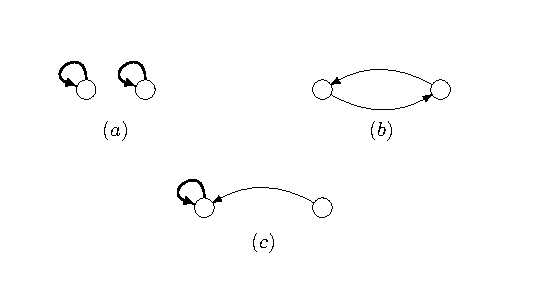
\includegraphics[scale=1.3]{figurenetworks.pdf}
\caption{Set of all possible networks with $N=2$ and $K=1$.}
\label{fig:rb}
\end{figure}

Topologies (a) and (b) have each the statistical weight $1/4$ in
the ensemble, since each of the links is connected in the
given way with probability $1/2$. Topology (c) has the
weight $1/2$, since there are two possibilities for realizing
this topology: either of the two nodes can be the one
with the self-link.


While the number of inputs of each node is fixed by
the parameter $K$, the number of outputs (i.e. of outgoing links) varies between the nodes. The mean number of
outputs must be $K$, since there must be in total the same
number of outputs as inputs. A given node becomes the
input of each of the N nodes with probability $\frac{K}{N}$ . In
the thermodynamic limit $N \to \infty$ the probability distribution of the number of outputs is therefore a Poisson
distribution:

$$
P_{out}(k) = \frac{K^k}{k!}e^{-K}
$$

\section{Dynamics}

All nodes are updated at the same time
according to the state of their inputs and to their update
function. Starting from some initial state, the network
performs a trajectory in state space and eventually arrives on an \emph{attractor}, where the same sequence of states
is periodically repeated. Since the update rule is deterministic, the same state must always be followed by the
same next state. If we represent the network states by
points in the $2^N$-dimensional state space, each of these
points has exactly one “output”, which is the successor
state. We thus obtain a graph in state space.
The size or length of an attractor is the number of
different states on the attractor. The basin of attraction
of an attractor is the set of all states that eventually
end up on this attractor, including the attractor states
themselves. The size of the basin of attraction is the
number of states belonging to it. The graph of states
in state space consists of unconnected components, each
of them being a basin of attraction and containing an
attractor, which is a loop in state space. The transient
states are those that do not lie on an attractor. They are
on trees leading to the attractors.


Let us illustrate these concepts by studying the small
$K = 1$ network shown in Figure~\ref{fig:rb2}, which consists of 4
nodes:

\begin{figure}[h]
\centering
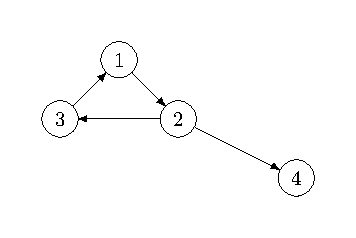
\includegraphics[scale=1.4]{figurenetworks2.pdf}
\caption{\emph{A small network with $N=4$ and $K=1$.}}
\label{fig:rb2}
\end{figure}

If we assign to the nodes 1,2,3,4 the functions invert,
invert, copy, copy, an initial state $1111$ evolves in the
following way:

$$
1111 \to 0011 \to 0100 \to 1111
$$

This is an attractor of period 3. If we interpret the bit se-
quence characterizing the state of the network as a number in binary notation, the sequence of states can also be
written as

$$
15 \to 3 \to 4 \to 15
$$

The entire state space is shown in Figure~\ref{fig:rb3}:
\begin{figure}[h]
\centering
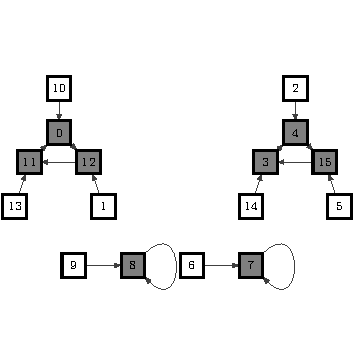
\includegraphics[scale=1.4]{fg3.pdf}
\caption{\emph{The state space of the network shown in Figure~\ref{fig:rb2}, if
the functions copy, copy, invert, invert are assigned to the four
nodes. The numbers in the squares represent states, and arrows indicate the successor of each state. States on attractors
are shaded.}}
\label{fig:rb3}
\end{figure}



There are 4 attractors, two of which are fixed points
(i.e., attractors of length $1$). The sizes of the basins of
attraction of the 4 attractors are $\Omega_1=6,\Omega_2= 6,\Omega_3 = 2,\Omega_4 = 2$. If the function
of node 1 is a constant function, fixing the value of the
node at 1, the state of this node fixes the rest of the
network, and there is only one attractor, which is a fixed
point.
\section{Phase transitions}
In RBNs, as well as in many dynamical systems, three
phases can be distinguished: \emph{ordered, chaotic, and critical} \cite{K19}.
These phases can be identified with different methods, since
they have several unique features.
these dynamical phases is related to
“sensitivity to initial conditions”, “damage spreading”, and
“robustness to perturbations” which are different ways of
measuring the stability of a network. We can “mutate”,
“damage” or “perturb” a node of a RBN by flipping its state.
We can also change a connection between two nodes, or in
the lookup table of a node. Since nodes affect other nodes,
we can measure how much a random change affects the rest
of the network. In other words, we can measure how the
damage spreads. This can be done by comparing the evolution of a “normal” network and a “perturbed” network. In
the ordered regime, usually the damage does not spread: a
“perturbed” network “returns” to the same path of the “normal” network. This is because changes cannot propagate
from one green island to another. In the chaotic phase, these
small changes tend to propagate through the network, making it highly sensitive to perturbations \cite{K49}.
An other feature is the convergence versus divergence of the
trajectories in state space of the network dynamics. In the ordered phase, similar states tend to converge to the same state.
In the chaotic regime, similar states tend to diverge. At the
edge of chaos, nearby states tend to lie on trajectories that
neither converge nor diverge in state space.
Living systems, or computing systems, need certain stability to survive, or to keep information; but also flexibility
to explore their space of possibilities. This has lead people
to argue that life and computation occur more naturally at
the edge of chaos or at the ordered regime
close to the edge of chaos \cite{K6}\cite{K49}.
\begin{figure}[h]
\centering
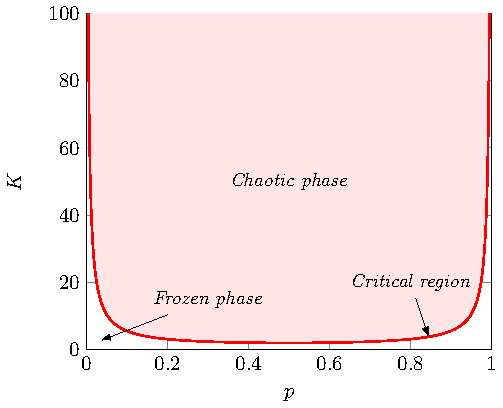
\includegraphics[scale=1.2]{images/phase-transition.pdf}
\caption{\emph{Phase diagram for the $N-K$ model. The shaded area corresponds
to the chaotic phase, whereas the white region corresponds to the chaotic phase.
The curve separating both regions is the critical phase.}}
\label{fig:ph-tr}
\end{figure}

Very early in the studies of
RBNs, people realized in simulations that the networks with
$K \le 2$ were in the ordered regime, and networks with $K \ge 3$,
were in the chaotic regime. In Figure \ref{fig:ph-tr} we can appreciate
characteristic dynamics of RBNs in different phases.
We can identify phase transitions in RBNs in different
ways. The main idea is to measure the effect of perturbations, the sensitivity to initial conditions, or damage spreading. This is analogous to Lyapunov exponents in continuous
dynamics.
The phase transitions can be statistically or analytically
obtained. Derrida and Pomeau were the first to determine
analytically that the critical phase (edge of chaos) was found
when $K = 2$ \cite{K8}\cite{K17}\cite{K21}.
following the model of Kauffman, RBN which most represent biological GRNs are those wich has $K=2$ \cite{K6}, because in the frozen phase (where $K=1$) networks are too simple to represent real regulatory networks; while in the caothic phase (where $K=3$) the time scales of the networks cycles grow exponentially, which is not biologically pheasible.
In Chapter \ref{analysis} we will see the differences in $K=1$ networks and $K=2$ networks.

\section{Attractor jumps}
In Kauffman model, attractors in the state space are considered as gene regulatory networks of different cells, where different attractors represent cells of different type, and where for example cancer cells lay in one specific attractor \cite{K3}\cite{K2}.
Now, if we suppose that different cell types lay in different attractors, we  suppose that the jump from an attractor to one other is given by a perturbation in the binary sequence of the genes.
So for example we take the previous network, and consider that we are in the state $12$ of the first attractor:
$$
12 \to 11 \to 0 \to 12
$$

And suddenly we change the state of the third node from $0$ to $1$:
$$
1100 \to 1110
$$

We change the system to have the state $14$ and so we jump into the second attractor:
$$
14 \to 3 \to 4 \to 15 \to 3
$$
\begin{figure}[h]
\centering
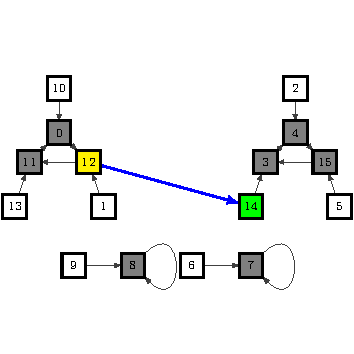
\includegraphics[scale=1.4]{fg4.pdf}
\caption{\emph{Jump from one attractor to one other in the state space.}}
\label{fig:rb4}
\end{figure}

So the branching pathways of differentiation between
attractors in a RBN in the ensembles create a directed
graph showing which attractors can be perturbed to reach which attractors.

In fact, if we consider all the possible stochastic perturbations in the binary sequence of the genes, we can get the all the possible transitions between the attractors, and what we obtain is an other network, where the nodes are the attractors and the frequencies of transitions can be used to build a random walk on this network\cite{K2}\cite{K3}\cite{K29}.



\chapter{Cancer attractors}
\lhead[\fancyplain{}{\bfseries\thepage}]{\fancyplain{}{\bfseries\rightmark}}

%\newcommand{\folder}{/path/to/folder}
\newenvironment{sistema}%
{\left\lbrace\begin{array}{@{}l@{}}}%
{\end{array}\right.}
In questo capitolo viene fatta una piccola introduzione al modello classico preda-predatore di Lotka-Volterra.
\section{The model}
We consider a physical system that can be described by an weighted interaction network among nodes that can assume different
dynamical states (in the case of a gene network the states $\sigma\in [0,1]$ and we have models similar to spin models).
In the simplest case, we introduce a stochastic dynamics using the probability $p_i(t)$ that the node $i$ is in the state $\sigma_i=1$
(then $1-p_i(t)$ is the probability to get $\sigma_i=0$) and we define a linear equation for the probability evolution
\begin{equation}
\dot p_i(t)=\sum_j \mathcal{P}_{ij}p_j(t)-\gamma_i p_i(t)
\label{average}
\end{equation}
where $\mathcal{P}_{ij}$ are transition probability rates and $\gamma_i^{-1}$ defines the mean lifetime of the excited state.
The meaning of the rates $\mathcal{P}_{ij}$ is the rate at which the excited state of the node $j$ increases (or decreases if
$\mathcal{P}_{ij}<0$) the probability of a transition to the excited state of the node $i$. Since $0\le p_i\le 1$ for all $i$, this space should be invariant for the dynamics. This condition depends on the spectral properties of the matrix
\begin{equation}
\mathcal{P}_{ij}-\gamma_j\delta_{ij}
\label{matrix}
\end{equation}
associated to the system. Let consider the case $\mathcal{L}_{ij}\ge 0$ (i.e. we have no inhibitory link),
the first quadrant is clearly invariant and if we define
$$
\sum_i  \mathcal{P}_{ij}=\hat \gamma_j>0
$$
the matrix 
$$
\mathcal{L}_{ij}=\mathcal{P}_{ij}-\hat \gamma_j \delta_{ij}
$$
is a Laplacian matrix and the system (\ref{average}) can be written in the form
$$
\dot p_i(t)=\sum_j \mathcal{L}_{ij}p_j(t)-\Delta \gamma_i p_i(t)\qquad \Delta \gamma_i=\gamma_i-\hat \gamma_i
$$
and by assumption we have $\gamma_i>\hat \gamma_i$. The eigenvalues of the matrix $\mathcal{L}_{ij}$
have all negative real part except the null eigenvalue. It follows that all the eigenvalue of the matrix (\ref{matrix})
has negative real part and the dynamics is a contraction towards the origin:
a stable solution (i.e. without any external stimulus the system relaxes to the $\sigma_i=0$ state).
A non trivial stationary can be achieved only if an external stimulus is inserted
\begin{equation}
\dot p_i(t)=\sum_j \mathcal{P}_{ij}p_j(t)-\gamma_i p_i(t)+\epsilon f_i(t)
\label{average_ext}
\end{equation}
The stationary solution has to satisfy $p_i\in [0,1]$ so that $f_i(t)\ge 0$ otherwise we can have negative probability 
when $p_i\simeq 0$. The case of a Laplacian matrix
$$
\hat \gamma_i=\gamma_i
$$
we get another possible stationary solution for $\mathcal{L}_{ij}p^\ast_j=0$ in the first quadrant and
the subspace $\sum p_i=0$ is invariant and the dynamics is a contraction in this subspace (in general).
Then the system a stable stationary solution even in absence of an external stimulus.\par\noindent
The presence of inhibitory links complicates the model and one has to prove that
\begin{itemize}
\item 1) there exists a physical space: an invariant cone in the first quadrant where the dynamics is a contraction towards
the origin;\par
\item 2) the external stimulus maintains the solution in the physical space.
\end{itemize}
Another solution could be to introduce boundary conditions so that $p_i\ge 0$ in any case (the system is non linear in such a case).
\par\noindent
The eigenvalues of the matrix (\ref{matrix}) define the different relaxation time scale the process and determine its rectivity
to the change of the external stimulus: in a typical problem one consider a slowly varying external stimulus so that the
system could be considered i a quasi stationary state
$$
\sum_j \mathcal{L}_{ij}p_j-\Delta \gamma_i p_i=-\epsilon f_i(t) \qquad \frac{df_i}{dt}\ll 1
$$
the derivative is small with respect to the eigenvalues of th matrix (adiabatic approximation). On the other hand we have the effect
of a correlated noise (we need to introduce a correlation in order have a continuous function $f_i(t)$). The problem is to
study the relation between the solution and the spectral properties of the matrix $\mathcal{L}_{ij}$: we simplify the
equation by assuming $\Delta \gamma_i=\Delta \gamma$ so that if $\lambda$ is an eigenvalue of $\mathcal{L}_{ij}$
then $\lambda-\Delta \gamma$ is an eigenvalue of the matrix (\ref{matrix}) and we assume that the dynamics
is perturbed by
\begin{equation}
\dot p_i(t)=\sum_j\left ( \mathcal{L}_{ij}+\Delta \mathcal{L}_{ij}\right ) p_j(t)-\Delta \gamma p_i(t)+\epsilon f_i(t)
\label{average_p}
\end{equation}
where the perturbation $\Delta\mathcal{L}_{ij}$ is a Laplacian matrix ($\sum_i \Delta\mathcal{L}_{ij}=0$ and we
assume $<\mathcal{L}>=0$) that can
represent an error in the measure of the transition rates $\mathcal{L}_{ij}$ or possible evolution of network due to
in time. In the first case we have an ensemble of transition matrices and we have to study the eigenvalue distribution
due to perturbation and the possible presence of bifurcation phenomena. In the second case we have a stochastic 
differential equation (since $\Delta \mathcal{L}_{ij}(t)$ can be represented as a realization of a stochastic process).
The possible approach are Perturbation Theory, Random Matrix Theory and Statistical Physics Methods for random matrices.
The external signal form the environment  (the environmental node) can be considered in the adiabatic approximation
(to be justified form a biological point of view).\par\noindent
The underlying stochastic process on the graph is defined by assigning the state $\xi_i(t)\in [0,1]$ at each node $i$ according 
to a probability distribution $\pi_i(t)$ that evolves as
$$
\dot \pi_i(t)=\sum_j \mathcal{L}_{ij}\xi_j(t)-\Delta \gamma \xi_i(t)+\epsilon f_i(t)
$$
By discretizing the dynamics for a time step $\Delta t$ we have the evolution
$$
\pi_i(t+\Delta t)=\pi(t)+\sum_j \mathcal{L}_{ij}\xi_j(t)\Delta t-\Delta \gamma \Delta t\xi_i(t)+\epsilon f_i(t)\Delta t
$$
and $\xi(t+\Delta t)$ realized according to the distribution $\pi_i(t+\Delta t)$ (stochastic cellular automata).
The average dynamics is computed by
\begin{eqnarray}
\dot <\pi_i(t)>&=&\sum_j \mathcal{L}_{ij}<\xi_j(t)>-\Delta \gamma <\xi_i(t)>+\epsilon f_i(t)\nonumber \\
&=&\sum_j \mathcal{L}_{ij}p_j(t)-\Delta \gamma p_i(t)+\epsilon f_i(t)=\dot p_i(t)\nonumber
\end{eqnarray}
and we recover the average equation (\ref{average}). But the stochastic dynamics gives information on the applicability
of the average approximation and the variability at the critical states (at bifurcation of the spectrum of $\mathcal{L}$).
The stochastic dynamics can be studied for stochastic connection matrices $\mathcal{L}+\Delta \mathcal{L}$.



\pagestyle{plain}


\chapter*{Appendix A}

\section*{Approssimazione di campo medio}


\begin{thebibliography}{90}             %crea l'ambiente bibliografia
\rhead[\fancyplain{}{\bfseries \leftmark}]{\fancyplain{}{\bfseries
\thepage}}
%%%%%%%%%%%%%%%%%%%%%%%%%%%%%%%%%%%%%%%%%aggiunge la voce Bibliografia
                                        %   nell'indice
\addcontentsline{toc}{chapter}{Bibliography}
%%%%%%%%%%%%%%%%%%%%%%%%%%%%%%%%%%%%%%%%%provare anche questo comando:
%%%%%%%%%%%\addcontentsline{toc}{chapter}{\numberline{}{Bibliografia}}

\bibitem{K13} Waddington CH, \emph{The strategy of the genes: a discussion of some aspects of theoretical biology}. London: Allen and Unwin, (1957)
\bibitem{K10} Cameron P. Gallivan, Honglei Ren and Elizabeth L. Read,\emph{Analysis of Single-Cell Gene Pair
Coexpression Landscapes by
Stochastic Kinetic Modeling Reveals
Gene-Pair Interactions in
Development},doi: 10.3389/fgene.2019.01387 ,(2019)

\bibitem{K11} Jifan Shi, Tiejun Li , Luonan Chen, Kazuyuki Aihara,\emph{Quantifying pluripotency landscape of cell
differentiation from scRNA-seq data by
continuous birth-death process},https://doi.org/10.1371/journal.
pcbi.1007488 ,(2019)
\bibitem{K12} Jin Wang, Kun Zhang, Li Xu, and Erkang Wang ,\emph{Quantifying the Waddington landscape and biological
paths for development and differentiation}, https://doi.org/10.1073/pnas.1017017108 ,(2011)

\bibitem{K4} S. Huang, I. Ernberg, S. Kauffman,\emph{Cancer attractors: A systems view of tumors from a gene network
dynamics and developmental perspective}, doi:10.1016/j.semcdb.2009.07.003, (2009)
\bibitem{K1} S. A. Kauffman, \emph{Metabolic Stability and Epigenesis in
Randomly Constructed Genetic Nets}, J. Theoret. Biol. (1969)
\bibitem{K5} Drossel B.,\emph{Random Boolean Networks},arXiv:0706.3351 ,(2008)
\bibitem{K3} R.Serra, M. Villani, A. Barbieri, S.A. Kauffman, A. Colacci,\emph{On the dynamics of random Boolean networks subject to noise:
Attractors, ergodic sets and cell types.},J Theor Biol 265: 185–193, (2010)
\bibitem{K2} M. Villani, A. Barbieri, R. Serra,\emph{A Dynamical Model of Genetic Networks for Cell Differentiation}, doi:10.1371/journal.pone.0017703.g001,(2011)
\bibitem{K9} M. Ali Al-Radhawi , Nithin S. Kumar, Eduardo D. Sontag , Domitilla Del Vecchio, \emph{Stochastic multistationarity in a model of the hematopoietic
stem cell differentiation network},doi:10.1109/cdc.2018.8619300, (2018)
\bibitem{K39} Janeway, \emph{Immunobiology}, 9th Edition
\bibitem{K40} E. Davidson, M. Levine, \emph{Gene Regulatory Networks}, doi:10.1073/pnas.0502024102, (2005)
\bibitem{K37} Chen L et al., \emph{Biomolecular networks: methods and applications in systems biology}, Wiley, Hoboken ,(2009)
\bibitem{K43} Peccoud, J. and Ycart, B., \emph{Markovian Modelling of Gene Products Synthesis.}, https://doi.org/10.1006/tpbi.1995.1027, (1995)
\bibitem{K44} T.B. Kepler and T.C. Elston, \emph{Stochasticity in transcriptional regulation: origins, consequences, and mathematical representations}, 10.1016/S0006-3495(01)75949-8 , (2001)
\bibitem{K45} J.M. Pedraza, J. Paulsson, \emph{Effects of molecular memory and bursting on fluctuations in gene expression}, 10.1126/science.1144331, (2008).
\bibitem{K46} Y. Sasai \emph{Cytosystems dynamics in self-organization of tissue architecture}, https://doi.org/10.1038/nature11859, (2013)
\bibitem{K47} B. Zhang and P. G. Wolynes, \emph{Stem cell differentiation as a many-body problem}, https://doi.org/10.1073/pnas.1408561111, (2014)
\bibitem{K48} Zhou et al., \emph{Fast Pyrolysis of Glucose-Based Carbohydrates withAdded NaCl Part 2: Validation and Evaluation of theMechanistic Model},DOI 10.1002/aic.15107, (2016)
\bibitem{K41} A. Wuensche, \emph{Genomic regulation modeled as a network with basins of attraction}, Pacific Symposium on Biocomputing. Pacific Symposium on Biocomputing, (1998)
\bibitem{K49} S. A. Kauffman, \emph{Investigations}, Oxford University
Press, (2000)
\bibitem{K42} MacArthur S. et al., \emph{Developmental roles of 21 Drosophila transcription factors are determined by quantitative differences in binding to an overlapping set of thousands of genomic regions},doi:10.1186/gb-2009-10-7-r80 (2009)
\bibitem{K7} S. A. Kauffman: J. Theor. Biol., 44, Physica D, 10, 145 (1984)
\bibitem{K6} S. Kauffman, \emph{A proposal for using the ensemble approach to understand
genetic regulatory networks},Journal of Theoretical Biology 230 (2004) 581–590 ,(2004)
\bibitem{K8} B. Derrida, \emph{Random Networks of Automata: A Simple Annealed
Approximat ion.}, (1985)
\bibitem{K17} B. Derrida and H.Flyvbjerg, \emph{The random map model: a disordere model with deterministic dynamics}, J.Physique, (1987)
\bibitem{K21} B. Derrida, \emph{Spin glasses, random boolean networks and simple models of evolution}

\bibitem{K50} C.W. Gardiner, \emph{Handbook of Stochastic Methods}, Springer, (1985)
\bibitem{K26} Sui Huang , Ingemar Ernberg, and Stuart Kauffman,\emph{Cancer attractors: A systems view of tumors from a gene network
dynamics and developmental perspective}, DOI:10.1016/j.semcdb.2009.07.003, (2009)














\bibitem{K15} M. Rybarsch and S. Bornholdt,\emph{On the dangers of Boolean networks:
Activity dependent criticality and threshold networks not faithful to biology}, arXiv:1012.3287v1. (2010)
\bibitem{K16} J. Park and M. E. J. Newman,\emph{The statistical mechanics of networks}, DOI: 10.1103/PhysRevE.70.066117 (2004)
\bibitem{K17} C. Gershenso,\emph{Introduction to Random Boolean Networks}, arXiv:nlin/0408006,(2004)

\bibitem{K19} R. V. Solè, B. Loque, \emph{Phase transitions and antichaos in generalized Kauffman networks},Physics Letters,(1994)
\bibitem{K20} J. T. Lizier, S. Pritam, M. Prokopenko, \emph{Information dynamics in small-world Boolean networks}, (2011)

\bibitem{K22} A. Rèka and A-L. Barabàsi, \emph{Statistical mechanics of complex networks}, Reviewes of modern physics, Volume 74,(2002)
\bibitem{K23} N. Masuda , M. A. Porter, R. Lambiotte ,\emph{Random walks and diffusion on networks},Physics Reports 716–717 1–58,(2017)
\bibitem{K24} T. Biyikoglu, J. Leydold, P. F. Stadler,\emph{Laplacian Eigenvectors of Graphs}, Springer
\bibitem{K25} Fan R. K. Chung,\emph{Spectral Graph Theory}, CBMS

\bibitem{K27} M. Ali Al-Radhawi, Nithin S. Kumar, Eduardo D. Sontag, Domitilla Del Vecchio ,\emph{Stochastic multistationarity in a model of the hematopoietic
stem cell differentiation network},DOI:10.1109/cdc.2018.8619300.,(2018)
\bibitem{K28} Rushina Shah, Domitilla Del Vecchio,\emph{Reprogramming cooperative monotone dynamical systems},DOI:10.1109/cdc.2018.8618649, (2018)
\bibitem{K29} Atefeh Taherian Fard and Mark A. Ragan, \emph{Modeling the Attractor Landscape of
Disease Progression: a
Network-Based Approach},DOI: 10.3389/fgene.2017.00048, (2017)
\bibitem{K30} Sui Huang, Yan-Ping Guo, Gillian May, Tariq Enver,\emph{Bifurcation dynamics in lineage-commitment in bipotent progenitor cells},Developmental Biology 305, (2007)
\bibitem{K31} Xin-She Yang and Young Z. L. Yang,\emph{Cellular Automata Networks},arXiv:1003.4958 , (2010)

\bibitem{K34} Xin Kang, Chunhe Li,\emph{Landscape inferred from gene expression data governs pluripotency in
embryonic stem cells},Computational and Structural Biotechnology Journal 18 (2020) 366–374,(2020)
\bibitem{K35} Genaro J. Martinez , Andrew Adamatzky  ,
Bo Chen , Fangyue Chen , Juan C.S.T. Mora ,\emph{Simple networks on complex cellular automata:
From de Bruijn diagrams to jump-graphs},(2017)



\bibitem{K38} Schnakenberg J., \emph{Network theory of microscopic and macroscopic behavior of master equation systems.}, Reviews of Modern Physics,Vol.48, (1976)



\end{thebibliography}
%%%%%%%%%%%%%%%%%%%%%%%%%%%%%%%%%%%%%%%%%non numera l'ultima pagina sinistra
\clearpage{\pagestyle{empty}\cleardoublepage}


\end{document}

